\documentclass[authordate, reflection]{jote-new-article}

\usepackage{caption}

\usepackage{tabularx}

\usepackage{graphicx}

\usepackage{hyperref}

\usepackage[backend=biber,style=apa]{biblatex}

\addbibresource{bibliography.bib}

\jotetitle{A Smiling Paradox: Exploring the Constructed Nature of Emotions. A Reflection on the Relationship Between Smiling in Selfies and Distress}
\keywordsabstract{facial expressions, emotion, selfie, emotion recognition}
\jname{Journal of Trial \& Error}
\jyear{2024}
\paperdoi{10.36850/4d60-44a8}
\paperreceived{July 15, 2024}
\author[1,2,3]{\mbox{Anne Margit Reitsema\orcid{0000-0002-7421-5907}}}
\affil[1]{Department of Developmental Psychology, Utrecht University}
\corremail{\href{mailto:a.m.reitsema@uu.nl}{a.m.reitsema@uu.nl}}
\corraddress{Utrecht University}
\runningauthor{Reitsema, Nijhof, \& Laceulle}
\author[2,3]{\mbox{Sanne Nijhof\orcid{0000-0003-1538-5014}}}
\affil[2]{Research Theme Dynamics of Youth, Thriving \& Healthy Youth, Utrecht University}
\author[1,2]{Odilia Laceulle}
\affil[3]{Department of Pediatrics, Wilhelmina Children’s Hospital, University Medical Center Utrecht, Utrecht University}
\paperaccepted{October 15, 2024}
\paperpublished{November 24, 2024}
\paperpublisheddate{2024-11-24}
\jwebsite{https://journal.trialanderror.org}

\specialissue{Scientific Failure and Uncertainty in the Health Domain}
\articletype{Scientific Failure - Reflection}

\begin{document}
\begin{frontmatter}
  \maketitle
  \begin{abstract}
    \printabstracttext
  \end{abstract}
\end{frontmatter}

 




	Much has been written about facial expressions and emotions, with numerous references pointing back to the world-famous studies conducted by Paul Ekman on universal expressions of emotion (see Figure 1). The work of Ekman and colleagues famously showed that even people from remote tribes in Papua New Guinea could recognize emotions from pictures of facial expressions (Ekman \& Friesen, 1969). This fostered the general belief that certain basic emotions -- six to be precise -- are part of our nature and shared universally. The study "Smile you're on camera: Investigating the relationship between selfie smiles and distress" (Lind et al., 2024) is one of many recent studies that challenge this fundamental emotion perspective. It urges us to consider a completely opposite view: Emotions are not universal but constructed through our cultural and personal experiences. Moreover, the study raises important questions on how much value society places on being -- or appearing -- happy, and the promises of AI powered emotion detection.




	\begin{figure}
		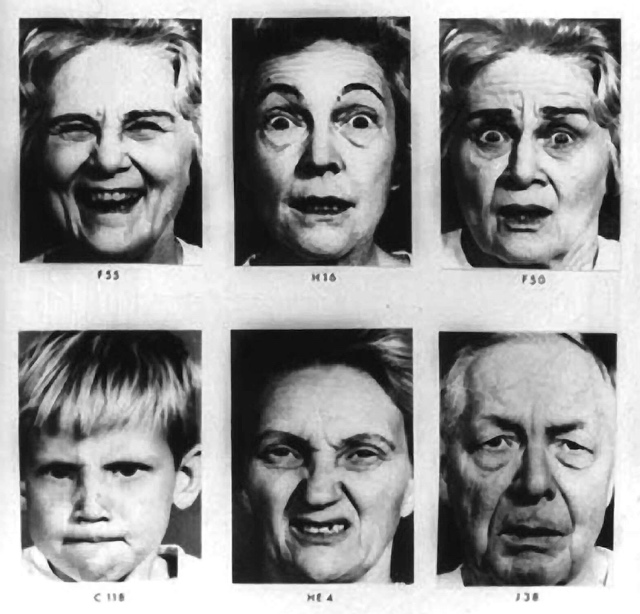
\includegraphics[width=\linewidth]{media/image1.jpeg}

		\caption{Photographs used in cross-cultural research by Ekman and Friesen (1969).}

		\label{fig:rId6}


	\end{figure}







	\section{The Study }



	In the current study (Lind et al., 2024), participants were asked to record daily two-minute videos in which they described one positive and one negative event from their day. Importantly, these videos were recorded in selfie mode, which means participants viewed themselves during the recording. The researchers subsequently used an automated facial behavior analysis toolkit to analyze the facial expressions in the videos. They focused on one specific so-called facial action unit that is commonly referred to the “lip corner puller”, also shown in the first photograph in Figure 1. While the researchers expected that more intense smiling would correlate with lower distress, their results showed the opposite pattern: Smiling intensity was associated with \emph{higher} levels of anxiety, depression, and stress. Although this may seem counterintuitive, these findings align with a growing body of research that shows that emotions are not universally and consistently experienced and expressed (Barrett et al., 2019). Instead, emotions might be \emph{constructed} based on a variety of factors, including past experiences and cultural norms.







	\section{Emotions in Context}



	The study's results, as the authors themselves also note, challenge Ekman's idea of discrete and universal “basic emotions”. We think it is valuable to reflect on this a bit deeper, since this idea still features prominently in many psychology textbooks and the popular press (e.g., American Psychological Association, 2018). A number of studies have now failed to replicate Ekman's findings (Barrett et al., 2019). The original Ekman study relied on forced-choice methods, which might have biased the results by priming participants with predetermined emotion categories. In studies that used a greater diversity of research methods, such as free sorting, people from remote tribes did not label the facial expressions as Ekman and his colleagues proposed, performing no better than chance (Gendron et al., 2018). These newer studies indicate that contextual factors play a much larger role in emotion perception than previously thought.



	According to the theory of constructed emotion (Barrett, 2017), emotions are not pre-set reactions that we are born with but are created by our brains on the spot by using a combination of bodily sensations, contextual information, and past experiences. To maximize efficiency and minimize energy use, our brains create emotions by using both past experiences and the current situation to predict to new situations. Instead of processing each experience “from scratch”, the brain efficiently reuses existing knowledge. This means that our emotions are very context-dependent: The same situation can evoke different emotions depending on an individual's prior experiences and the current environment.



	A range of studies support this constructed view of emotions by showing that things like facial expressions, autonomic responses, and brain activity do not form distinct, consistent clusters that can clearly differentiate one type of emotion from another (e.g., Lindquist et al., 2012; Siegel et al., 2018). Instead, variability is the norm. The same emotion can lead to different facial expressions depending on cultural expectations and personal history. For instance, when you are angry, your facial expression is not always the same and does not always look exactly as the expression in the fourth photograph in Figure 1. Sometimes you might frown when you are angry, other times you may cry, or you might show no obvious sign of anger at all if it is not appropriate for the situation. The expressions in Figure 1 are therefore better thought of as stereotypes that fail to capture the rich variety of emotion expressions that likely emerge in daily life.



	Applying the theory of constructed emotions to the current study provides valuable insights into the unexpected association between smiling intensity and higher distress. In the unique context of recording selfie videos, participants may construct emotions and expressions in ways that differ from everyday life. Participants that experience higher levels of anxiety or stress might construct their emotional response to include more intense smiling as a way to cope with or regulate their internal discomfort. Moreover, smiling intensely in this context could itself potentially contribute to feelings of distress, as participants become more self-aware and perhaps self-critical. This highlights the theory's core idea that emotional experiences and expressions are deeply shaped by context—what might appear to be a smile of happiness may, in fact, be a response to stress or anxiety.







	\section{Social Norms and Emotion}



	Social norms play a crucial role in shaping how emotions are expressed and interpreted. This is particularly relevant in the context of the current study, where participants were continually confronted with their own expressions while recording selfie videos. Lind and colleagues discussed this in the context of Fridlund's behavioral ecology view (1994), which proposes that facial expressions are better understood as tools for communication rather than direct reflections of a person's inner emotions. These communicative tools are heavily influenced by cultural norms, which dictate which emotions should be expressed or suppressed. Given that participants were more self-aware while recording themselves, they might have been influenced by these cultural norms, leading them to display emotions that do not necessarily reflect their true feelings.



	In many cultures, especially in Western societies, there is an emphasis on happiness and the maximization of positive emotions and minimization of negative ones (Bastian et al., 2015). There is often a societal expectation to always look happy, which can lead to frequent smiling and acting cheerful even when people do not feel that way, which ironically is linked to poorer well-being (Dejonckheere et al., 2022). This trend is particularly strong on social media where people predominantly share positive moments and emotions and downplay or omit negative ones. This can make the pressure to fit in with societal expectations even stronger. Moreover, the constant exposure to such idealized displays of happiness can lead to unrealistic social comparisons and negatively impact mood (Bennett et al., 2017).



	In the context of the original study, the societal expectation to display positive emotions, such as smiling, may be amplified by the artificial setting. The act of recording a selfie video may trigger awareness of social expectations, particularly the pressure to appear positive in self-presentations. This could lead participants to smile more intensely to conform to these social norms. Given our growing understanding of emotions as social and contextualized phenomena, future research should prioritize methods that capture this complexity. This could include, for example, more ecological momentary assessment research to study emotions in real-time natural settings, conducting cross-cultural studies to examine how social norms influence emotion construction and expression, and developing multimodal assessment techniques that combine facial expressions, physiological measures, and self-reports.







	\section{Practical and Ethical Considerations}



	Facial expression analysis, like the kind used in this study, is rapidly gaining popularity and is increasingly applied in many fields, including psychology. It is one of the primary methods used in emotion-detection technology, alongside voice analysis, gait analysis, and eye tracking. Many companies, including Affectiva (an MIT spin-off) and Hume AI (which recently received \$50 million in new funding, Business Wire, 2024), as well as tech giants like Apple, Google, and Facebook, are actively developing these technologies. These innovations are believed to provide companies with a competitive advantage and are already being implemented in diverse areas. For instance, they are used during job interviews to evaluate candidates' emotional responses (Unilever; Hymas, 2019), to predict the popularity of movies (Disney; Deng et al., 2017), and even for personalized menu recommendations in fast food (KFC; Hawkins, 2017).



	However, the keyword in all of this is \emph{accuracy}. The basis for emotion-recognition technology is just not there. After reviewing over 1,000 papers on facial expression of emotion, Barrett and colleagues (2019, p. 46) concluded: “It is not possible to confidently infer happiness from a smile, anger from a scowl, or sadness from a frown, as much of current technology tries to do when applying what are mistakenly believed to be the scientific facts.” This is similar to the flawed logic behind polygraphs or “lie detectors”: The assumption that we can directly infer people's mental states from their physical expressions. While these technologies can be very accurate at detecting facial expressions, they ultimately cannot tell us what these expressions mean or what the person is actually feeling.



	Will it then ever be possible to have accurate AI emotion detection? Maybe, but there are significant challenges to overcome. Right now, most AI technologies rely on simplified facial expressions to detect emotions, which -- as we saw -- does not capture the full picture (Barrett et al., 2019; Cabitza et al., 2022; Cross et al., 2023). For AI to get better at “reading” emotions, it needs to move past these stereotypes and recognize the variety of possible expressions and the context in which they occur. This means that other factors also need to be considered, like environment and time of day. For any AI to detect emotions accurately, it must understand the context in which expressions occur, as emotions are context-bound (Barrett, 2022). Detailed data from people in various real-life situations can allow for a more complete understanding of emotional expression. This involves using multiple types of data, like voice analysis and body posture, to get a fuller picture. By doing this, AI could better understand that a smile does not always mean someone is happy -- they might be smiling but in reality, feel stressed or upset.







	\section{Conclusion}



	The study's finding that intense smiling can signal distress highlights the complexity of emotions. It illustrates that expressions are influenced by context, shaped by social norms, and deeply intertwined with personal experiences. These findings challenge the traditional view that facial expressions are straightforward reflections of internal states. They also raise crucial questions for AI emotion-detection systems, which often simplify the interpretation of expressions. Moving forward, research should prioritize exploring emotions in real-world settings, using more refined methods that can capture their variability and complexity. By advancing our understanding of how context shapes emotional expression, both research and AI systems can move toward more accurate and holistic interpretations of emotional signals.











	\section{References}



	American Psychological Association. (2018). \emph{Primary emotion}. In \emph{APA Dictionary of }\emph{Psychology}. Retrieved July 15, 2024, from \url{https://dictionary.apa.org/primary-emotion}



	Barrett, L. F. (2017). The theory of constructed emotion: An active inference account of interoception and categorization. \emph{Social Cognitive and Affective Neuroscience, 12}, 1--23. \url{https://doi.org/10.1093/scan/nsw154}



	Barrett, L. F. (2022). Context reconsidered: Complex signal ensembles, relational meaning, and population thinking in psychological science. \emph{American Psychologist}, \emph{77}(8), 894-920. \url{https://doi.org/10.1037/amp0001054}



	Barrett, L. F., Adolphs, R., Marsella, S., Martinez, A. M., \& Pollak, S. D. (2019). Emotional expressions reconsidered: Challenges to inferring emotion from human facial movements. \emph{Psychological Science in the Public Interest}, \emph{20}(1), 1-68. \url{https://doi.org/10.1177/1529100619832930}



	Bastian, B., Koval, P., Erbas, Y., Houben, M., Pe, M., \& Kuppens, P. (2015). Sad and alone: Social expectancies for experiencing negative emotions are linked to feelings of loneliness. \emph{Emotion, 6}(5), 496--503. \url{http://doi.org/10.1177/1948550614568682}



	Bennett, B. L., Whisenhunt, B. L., Hudson, D. L., Wagner, A. F., Latner, J. D., Stefano, E. C., \& Beauchamp, M. T. (2020). Examining the impact of social media on mood and body dissatisfaction using ecological momentary assessment. \emph{Journal of American College Health}, \emph{68}(5), 502-508. \url{https://doi.org/10.1080/07448481.2019.1583236}



	Business Wire. (2024, March 27). \emph{Hume AI announces \$50 million fundraise and empathic } \emph{voice interface}. Business Wire. \url{https://www.businesswire.com/news/home/20240326359639/en/Hume-AI-Announces-50-Million-Fundraise-and-Empathic-Voice-Interface}



	Cabitza, F., Campagner, A., \& Mattioli, M. (2022). The unbearable (technical) unreliability of automated facial emotion recognition. \emph{Big Data \& Society}, \emph{9}(2). \url{https://doi.org/10.1177/20539517221129549}



	Cross, M. P., Acevedo, A. M., \& Hunter, J. F. (2023). A critique of automated approaches to code facial expressions: What do researchers need to know?. \emph{Affective Science}, \emph{4}(3), 500-505. \url{https://doi.org/10.1007/s42761-023-00195-0}



	Dejonckheere, E., Rhee, J. J., Baguma, P. K., Barry, O., Becker, M., Bilewicz, M., Castelain, T., Costantini, G., Dimdins, G., Espinosa, A., Finchilescu, G., Friese, M., Gastardo-Conaco, M. C., Gómez, A., González, R., Goto, N., Halama, P., Hurtado-Parrado, C., Jiga-Boy, G. M., … Bastian, B. (2022). Perceiving societal pressure to be happy is linked to poor well-being, especially in happy nations. \emph{Scientific Reports}, \emph{12}(1), Article 1514. \url{https://doi.org/10.1038/s41598-021-04262-z}



	Deng, Z., Navarathna, R., Carr, P., Mandt, S., Yue, Y., Matthews, I., \& Mori, G. (2017). Factorized variational autoencoders for modeling audience reactions to movies. In \emph{Proceedings of the IEEE conference on computer vision and pattern recognition} (pp. 2577-2586). \url{https://doi.org/10.1109/CVPR.2017.637}



	Ekman, P., Sorenson, E. R., \& Friesen, W. V. (1969). Pan-cultural elements in facial displays of emotion. \emph{Science}, \emph{164}(3875), 86-88. \url{https://doi.org/10.1126/science.164.3875.86}



	Fridlund, A. J. (1994). \emph{Human facial expression: An evolutionary view}. Academic Press.



	Gendron, M., Crivelli, C., \& Barrett, L. F. (2018). Universality reconsidered: Diversity in making meaning of facial expressions. \emph{Current Directions in Psychological Science}, \emph{27}(4), 211-219. \url{https://doi.org/10.1177/0963721417746794}



	Hawkins, A. (2017, January 11). \emph{KFC China is using facial recognition tech to serve } \emph{customers -- but are they buying it?} The Guardian. \url{https://www.theguardian.com/technology/2017/jan/11/china-beijing-first-smart-restaurant-kfc-facial-recognition}



	Hymas, C. (2019, September 27). \emph{AI facial recognition used for first time in job interviews in } \emph{UK to find best applicants}. The Telegraph. \url{https://www.telegraph.co.uk/news/2019/09/27/ai-facial-recognition-used-first-time-job-interviews-uk-find/}



	Lind, M. N., Byrne, M. L., Devine, S., \& Allen, N. B. (2024). Smile, you're on camera: Investigating the relationship between selfie smiles and distress. \emph{Journal of Trial \& Error}. \url{https://doi.org/10.36850/8716-5abe}



	Lindquist, K. A., Wager, T. D., Kober, H., Bliss-Moreau, E., \& Barrett, L. F. (2012). The brain basis of emotion: A meta-analytic review. \emph{Behavioral and Brain Sciences}, \emph{35}(3), 121-143. \url{https://doi.org/10.1017/S0140525X11000446}



	Siegel, E. H., Sands, M. K., Van den Noortgate, W., Condon, P., Chang, Y., Dy, J., Quigley, K. S., \& Barrett, L. F. (2018). Emotion fingerprints or emotion populations? A meta-analytic investigation of autonomic features of emotion categories. \emph{Psychological Bulletin}, \emph{144}(4), 343-393. \url{https://doi.org/10.1037/bul0000128}






\end{document}